\documentclass[12pt]{article}
\title{ECE M16 Homework 2}
\usepackage{subcaption}
\author{Lawrence Liu}
\usepackage{graphicx}
\usepackage{amsmath}
\usepackage{placeins}
\newcommand{\Laplace}{\mathscr{L}}
\setlength{\parskip}{\baselineskip}%
\setlength{\parindent}{0pt}%
\usepackage{xcolor}
\usepackage{listings}
\definecolor{backcolour}{rgb}{0.95,0.95,0.92}
\usepackage{amssymb}
\lstdefinestyle{mystyle}{
    backgroundcolor=\color{backcolour}}
\lstset{style=mystyle}

\begin{document}
\maketitle
\section*{HW1 Problem  4 part b}
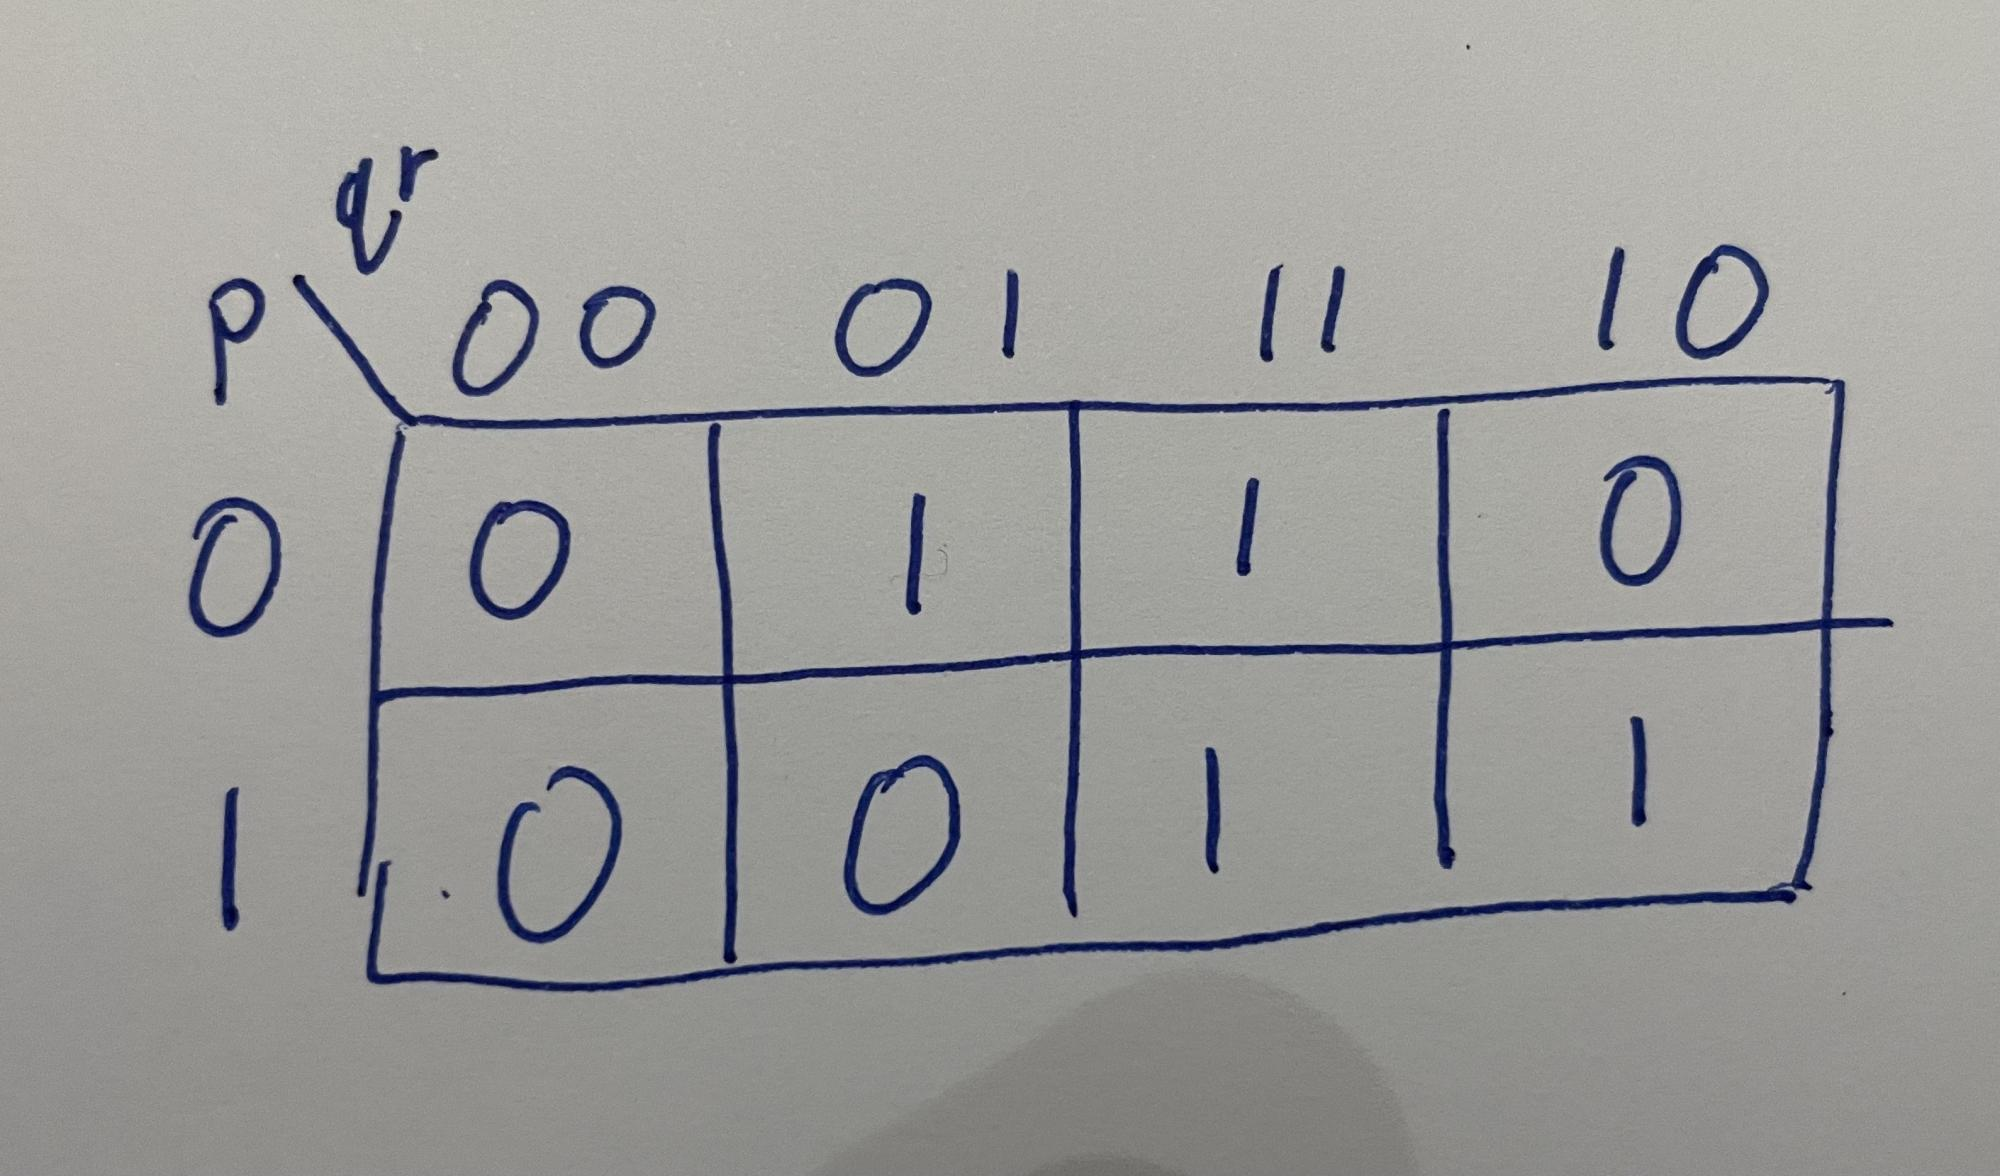
\includegraphics[scale=0.15]{../HW1/Kmap.jpg}
\section*{HW1 Problem 7}
\subsection*{(a)}
\begin{center}
    \begin{tabular}{|c|c|c|c|c|c|}
        Month & m3 & m2 & m1 & m0 & output \\
        \hline
        1 & 0 & 0 & 0 & 1 & 1 \\
        \hline
        2 & 0 & 0 & 1 & 0 & 0 \\
        \hline
        3 & 0 & 0 & 1 & 1 & 1 \\
        \hline
        4 & 0 & 1 & 0 & 0 & 0 \\
        \hline
        5 & 0 & 1 & 0 & 1 & 1 \\
        \hline
        6 & 0 & 1 & 1 & 0 & 0 \\
        \hline
        7 & 0 & 1 & 1 & 1 & 1 \\
        \hline
        8 & 1 & 0 & 0 & 0 & 1 \\
        \hline
        9 & 1 & 0 & 0 & 1 & 0 \\
        \hline
        10 & 1 & 0 & 1 & 0 & 1 \\
        \hline
        11 & 1 & 0 & 1 & 1 & 0 \\
        \hline
        12 & 1 & 1 & 0 & 0 & 1 \\
        \hline
    \end{tabular}
\end{center}
\subsection*{(b)}
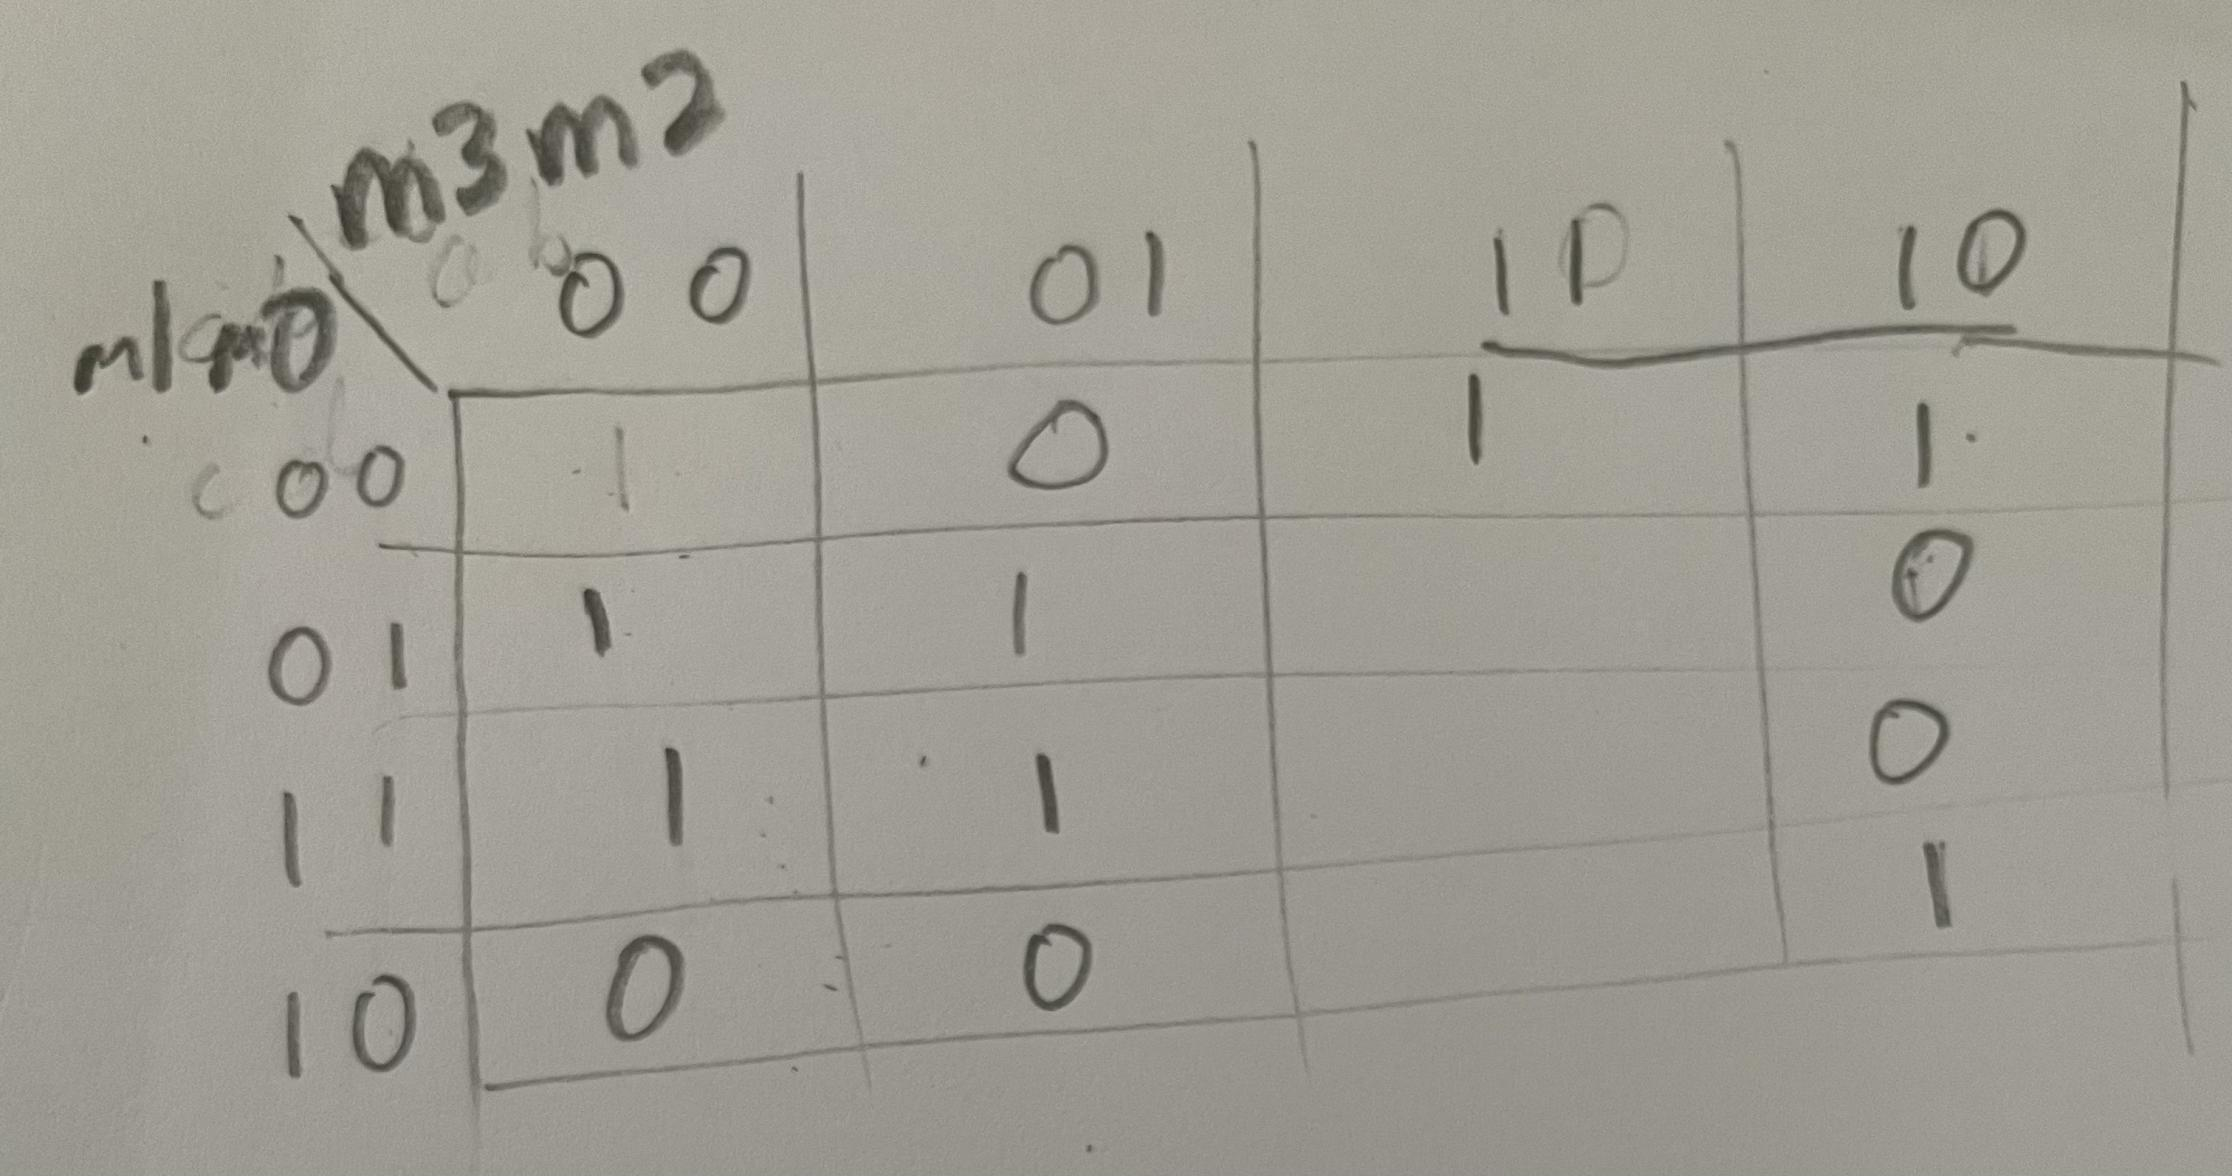
\includegraphics[scale=0.15]{Problem7Kmap.jpg}\\
Therefore the equation is:
$$\boxed{m_0.\overline{m_3}+\overline{m_0}.m3}$$
\subsection*{(c)}
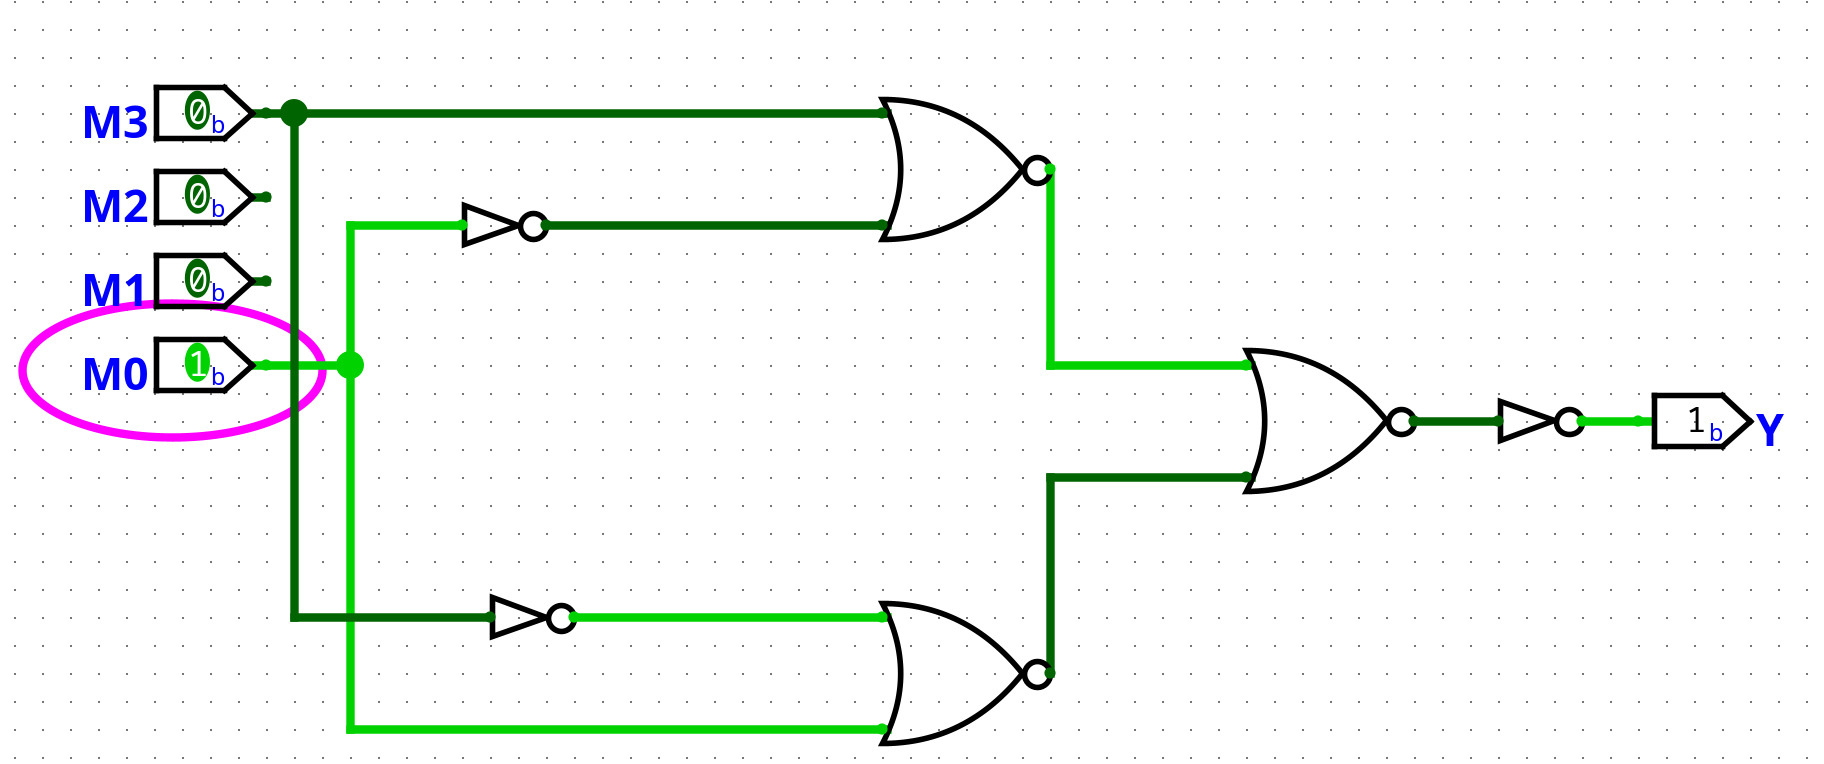
\includegraphics[scale=0.25]{Problem7Partc.png}
\section*{HW 2 Problem 1}

\end{document}